\documentclass[11pt,dvipdfmx,a4paper]{jsarticle}

\usepackage{amsmath,amssymb}
\usepackage{bm}
\usepackage[dvipdfmx]{graphicx}
\usepackage{physics} % http://mirrors.ibiblio.org/CTAN/macros/latex/contrib/physics/physics.pdf
\usepackage{siunitx} %SI単位を楽に出力
\usepackage{mathtools} %環境の追加
\usepackage{circuitikz} %電気回路をtex中で書く
% \usepackage{caption} %番号なしキャプションを書く
% \usepackage{cancel} %式中に斜線を入れる
% \usepackage{tensor} %テンソルの添え字を書く
% \usepackage{tikz} %図を書く
% \usepackage{ascmac} %四角い枠の中に文章を書く
% \usepackage{float} %figureで[hbp]オプションを使う
% \usepackage{hyperref}  \usepackage{pxjahyper} %ハイパーリンクをつかう
% \usepackage{tablefootnote} %表中に注釈をいれる
% \usepackage[thicklines]{cancel} %数式中の取り消し線
\usepackage[version=4]{mhchem} %化学式の入力
\usepackage{pdfpages}
\usepackage{wrapfig} %文章の回り込み
\usepackage[subrefformat=parens]{subcaption} %(a)図のようにすることができるやつ
\usepackage{here}
\usepackage{mathrsfs} % フォントの追加
\usepackage{url} % url を入れる
\usepackage[margin=15mm]{geometry} %余白の削除
\usepackage{tcolorbox}

\graphicspath{{./image/}}

\begin{document}

%出力したpdfを表紙にするとき
% \includepdf[pages=1,noautoscale=false]{cover.pdf}
% \newpage

%texで表紙を書くとき
\quad\\[35mm]
\centerline{\Huge{\textsf{第 7 回}}}
\quad\\[5mm]
\centerline{\Huge{\textsf{応 用 物 理 学 実 験}}}
\quad\\[5mm]
\begin{table}[h]
	\centering
	\begin{tabular}{| c | c |}
		\hline
		\Huge\textsf{{題目}} & \Huge{\textsf{強誘電体ヒステリシス曲線}} \rule[-5mm]{0mm}{15mm} \\
		\hline
	\end{tabular}
\end{table}
\quad\\[10mm]
\begin{table}[h]
	\centering
	\begin{tabular}{l l}
		\hline
		\LARGE{\textsf{氏\qquad 名}} & \LARGE{\textsf{: 西原 翔}} \rule[0mm]{0mm}{6mm} \\
		\hline
		\LARGE{\textsf{学  籍  番  号}} & \LARGE{\textsf{: 1522068}} \rule[0mm]{0mm}{6mm} \\
		\LARGE{\textsf{学部学科学年}} & \LARGE{\textsf{: 理学部第一部応用物理学科3年}}\\
		\hline
	\end{tabular}
\end{table}
\quad\\[10mm]
\centerline{\LARGE{\textsf{共同実験者:1522064 中井空弥}}}\\[2mm]
% \centerline{\LARGE{\textsf{\qquad\qquad\quad\;\;1522091 宮田祟杜}}}\\[2mm]
% \centerline{\LARGE{\textsf{\qquad\qquad\quad\;\;1522095 村山涼矢}}}\\[2mm]
% \centerline{\LARGE{\textsf{\qquad\qquad\quad\;\;1522B02 中村洸太}}}\\[2mm]
\quad\\[10mm]
\centerline{\LARGE{\textsf{提出年月日:2024年10月24日}}}\\[2mm]
\centerline{\LARGE{\textsf{実験実施日:2024年10月04日}}}\\[2mm]
\centerline{\LARGE{\textsf{\qquad\qquad\quad\;2024年10月11日}}}
\quad\\[10mm]
\centerline{\LARGE{\textsf{東 京 理 科 大 学 理 学 部 第 1 部}}}\\[2mm]
\centerline{\LARGE{\textsf{応 用 物 理 学 教 室}}}

\thispagestyle{empty}
\clearpage
\addtocounter{page}{-1}
\newpage

% \twocolumn

\section{Abstract}
強誘電体はその自発分極の向きによって情報を保存するメモリとしてや、コンデンサとして現在役立てられている。
この強誘電体の自発分極を持つという性質は温度を上げていくといずれ失われ、
自発分極を持たない常誘電体へと相転移する。
誘電体・強誘電体相転移をすることで知られる
\ce{BaTiO_3} (BTO) と \ce{(NH_2CH_2COOH)_3 H_2 SO_4} (TGS) の外部電場に対する電束密度の応答を
室温から相転移温度以上の温度の間で測定した。
BTO は直前の状態に依存して変わるヒステリシス現象を強誘電相・常誘電相、両方において示し、
TGS は強誘電相でのみ示した。
この応答の違いは強誘電性の起源となる仕組みが違うことを表している。
これらの振る舞いを結晶の対称性を反映した自由エネルギーを用いて議論する
ランダウ理論の示す結果と比較した。

\section{Introduction}
強誘電体は電場をかけずとも自発分極を持ち、また外部電場によってその向きを変えることができる。
これはつまり不揮発性メモリとして利用することができる。
またこれを用いたコンデンサはサイズに対する静電容量が大きくコンデンサとしての用途も期待できる。
さらに、強誘電体はその結晶構造によるところが大きく、ひずみよって分極が変わる。
これより圧力のセンサーとしても使うことができる素材である。
そのためこれまでにも強誘電体の性質やこれを応用したデバイスの研究が広く行われてきた。

そうした強誘電体は温度を上げていくと自発分極を持つという性質を失った常誘電体へと変化する。
この相転移の様子をかけた電場への応答という点から測定していく。

今回、変位型強誘電体の代表として BTO, 規則不規則型強誘電体の代表として TGS を測定した。
前者はセラミックコンデンサとして、後者は圧電センサーとして利用されている素材である。
これら素材の結晶学的な性質をまとめる。

\begin{figure}[H]
    \centering
    \begin{minipage}[t]{0.48\columnwidth}
        \centering
        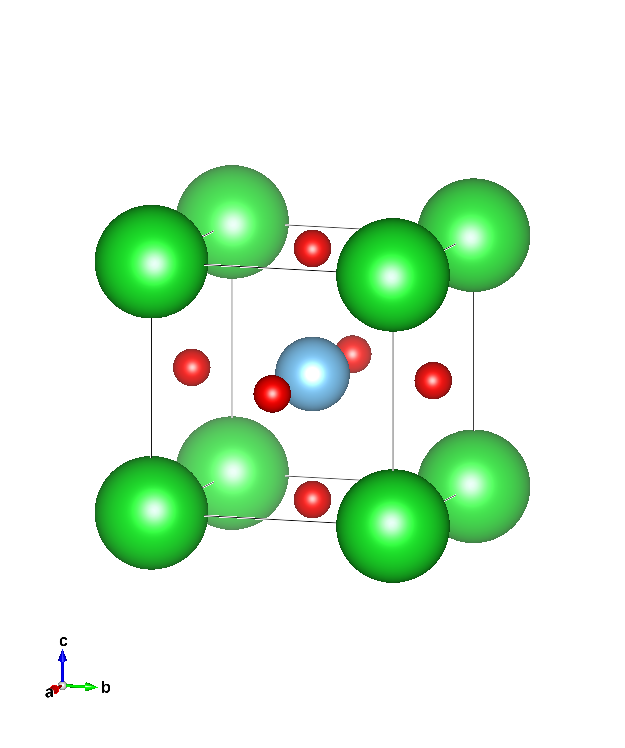
\includegraphics[width = \columnwidth]{BTO.png}
        \subcaption{\ce{BaTiO_3}の立方晶ペロブスカイト構造。
        空間群は $Pm\bar{3}m$, 格子定数は a = 4.04 \AA.
        緑色が Ba, 青色が Ti, 赤色が O を表している。}
        \label{structure:BTO}
    \end{minipage}
    \begin{minipage}[t]{0.48\columnwidth}
        \centering
        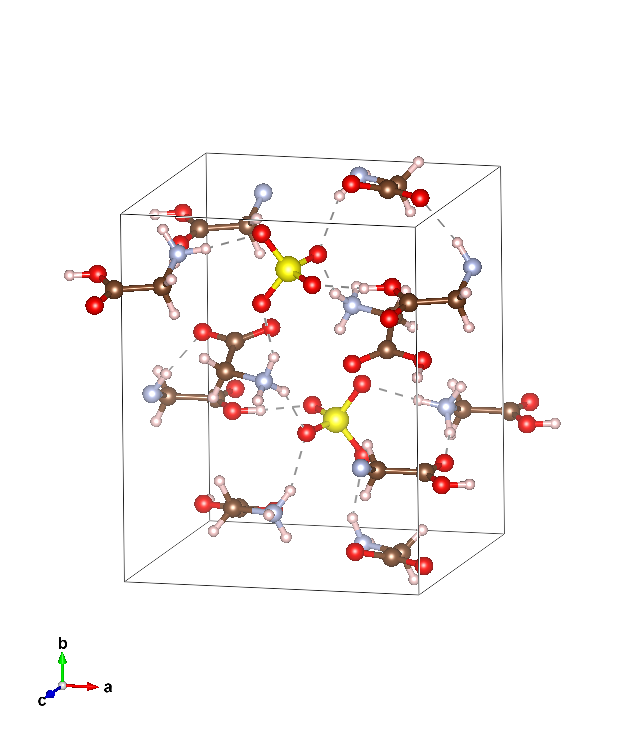
\includegraphics[width = \columnwidth]{TGS.png}
        \subcaption{\ce{(NH_2CH_2COOH)_3 H_2SO_4}の構造。
        空間群は $P2_1$, 格子定数は a = 9.44 \AA, b = 12.63 \AA, c = 5.71 \AA, $\beta$ = 110\si{\degree}.
        cif データ\cite{cif:7128310} をもとに作成した。
        黄色と赤色の四面体が硫酸イオン、
        その他の黒色と青色からなる構造がグリシンである。}
        \label{structure:TGS}
    \end{minipage}
    \caption{今回測定した試料の結晶構造。VESTA\cite{VESTA}を用いて作成した。}
\end{figure}

\subsection{試料の結晶構造}
\subsubsection*{\ce{BaTiO_3}}
\ce{BaTiO_3} はペロブスカイト型酸化物 \ce{ABO_3} の一種であり、BTO と略される。
理想的な立方晶ペロブスカイトの構造は金属原子 A が単位胞の各頂点、
金属原子 B が単位胞の体心位置、酸素 O が面心位置を占有しているような構造である(図\ref{structure:BTO})。
A 原子と B 原子を置換することで格子定数や電子密度を変えることができ、
物性を変え様々な機能を持たせることができる構造である。
ただ、構成する金属原子や環境の温度・圧力によっては \ce{BO_6} の正八面体が傾いたり歪みが生じ、
対称性の異なる結晶構造になる。
BTO は絶対零度の基底状態から温度を上げていくと順に
菱面体晶$(R3m)$, 斜方晶$(Amm2)$,
正方晶$(P4mm)$,
立方晶$(Pm\bar{3}m)$へと変化する。

\subsection*{\ce{(NH_2CH_2COOH)_3 H_2SO_4}}
\ce{(NH_2CH_2COOH)_3 SO_4} は TGS と略され、アミノ酸であるグリシン\ce{NH_2CH_2COOH} 3つと硫酸\ce{H_2SO_4}が集まったものである。(図\ref{structure:TGS})。
空間群は $P2_1$, 格子定数は a = 9.44 \AA, b = 12.63 \AA, c = 5.71 \AA, $\beta$ = 110\si{\degree} の単斜晶の結晶である。
これは b 軸方向に沿って硫酸イオンとグリシンの層、アミノ基にプロトンがくっついているグリシン2つの層が水素結合によって交互に積層している構造である。


\section{Methods}
\begin{wrapfigure}{r}[0pt]{0.35\columnwidth}
    \centering
    \begin{circuitikz}
        \draw (0, 0)
            to[tV, v=$V_i$] (0, 2)
            to[short] (2, 2)
            to[C=$C_x$] (2, 1)
            to[C=$C_s$] (2, 0)
            to[short] (0, 0);
        % \draw (2, 1)
        %     to[short, -o] (3, 1)
        %     node[anchor=west]{Ch. 2};
        \draw (-0.5, 1.5)
            node[anchor=south]{50Hz};
        \draw(0,0) to node[ground]{} ++(0,0);
    \end{circuitikz}
    \caption{電場に対する試料の電束密度の応答を調べる回路(Sawyer-Tower 法)。
    $C_x$がサンプルの静電容量、$C_s$は標準コンデンサの静電容量。
    入力は 50 Hz の三角波。オシロスコープの Ch.1 で入力三角波の電圧を、
    Ch.2 で$C_s$の両端の電圧差を測定することで試料にかけた電場\(E\)に対する応答である電束密度\(D\)を測定できる。}
    \label{fig:circuit}
\end{wrapfigure}
試料に\(E\)の電場をかけたときの試料中の電束密度\(D_x\)の大きさを測定する回路の模式図は図\ref{fig:circuit}である。
実際にはアンプ等が入っているが物理量の測定の仕組みにかかわる部分を抜き出してある。
\(C_x\)がサンプルの静電容量、\(C_s\)が標準コンデンサの静電容量で\(C_s\gg C_x\)になるように標準コンデンサを選んである。
50 Hz の三角波を入力として、これを記録するためにオシロスコープの Ch.1 で記録する。
この 50 Hz の周期的な入力ではあるが、誘電体の配向分極と共鳴する振動数は 1kHz 程度のオーダーである(2OB 実験:複素インピーダンス測定)
のでこの入力は直流入力だとみなすことができる。
また、\(C_s\)の両端の電圧差をオシロスコープの Ch.2 で記録をする。
このとき、試料にかかる電圧はオシロスコープの各チャンネルに入力される電圧を\(V_{\text{Ch.1}}, V_{\text{Ch.2}}\)とすると、
コンデンサ回路の電荷保存則より試料にかかる電圧\(V_x\)と標準コンデンサにかかる電圧\(V_{\text{Ch.2}}\)は
\begin{align}
    V_x &= \frac{C_s}{C_s+C_x}V_{\text{Ch.1}} \simeq V_{\text{Ch.1}}\\
    V_{\text{Ch.2}} &= \frac{C_x}{C_s+C_x}V_{\text{Ch.1}} \simeq \frac{C_x}{C_s}V_x
\end{align}
というように書ける。ここでコンデンサ表面の電荷と電束密度の間のガウスの法則により、
平行版コンデンサの面積を\(A\)として
\begin{align}
    C_x V_x = Q_x = D_x A
\end{align}
というように書ける。
そして試料にかかっている電場の大きさは平行版コンデンサの厚さを\(d\)として\(E = V/d\)と書ける。
これらをまとめると
\begin{align}
    E = \frac{1}{d}V_{\text{Ch.1}}, \qquad
    D_x = \frac{C_s}{A}V_{\text{Ch.2}}
\end{align}
というようになり、オシロスコープのXYモードで表示させることで
試料に電場\(E\)をかけたときの試料中の電束密度\(D_x\)の関係を表示・記録することができるのがわかる。

電束密度\(D_x\)の温度依存性を見るため、実際の系では\(C_x\)は熱電対温度計と共に炉の中に入れ測定した。


\section{Results (TGS)}
TGS に自発分極の向きである [010] 方向に電場を加えたときの電束密度の振る舞いの測定結果を見ていく。
ただし、ここでのデータはオシロスコープの測定ノイズやバルクハウゼン効果を無視するため、
移動平均を取って平均値が0になるように平行移動をしてある。
図\ref{graph:TGS_D-E_Ec}は試料を特定の温度に保ったまま、入力電場の最大値を変えたときのヒステリシス曲線の様子である。
電場の最大値が小さいときにはヒステリシス曲線の形が平行四辺形のような形からなめった形となっている。
試料の自発分極の向きが入力電場の向きと揃うことなく電場が小さくなってしまうことが原因と考えられる。
どれほど最大電場がどれほどの電場をかければよいかを考える。
自発分極が入力電場と揃うのに必要な電場の強さは一定であるため、
十分な電場がかかっているときには保持電場と最大電場の比\(E_C/E\)は徐々に小さくなっていく。
実際にこれをプロットしたのが図\ref{graph:TGS_Ec-E}である。
点線を境目に\(E_c/E\)の値の変化の仕方が変わっていることから、
TGS でヒステリシス曲線を見るとなったときには 5 kV/cm 以上の電場をかければよいとわかる。
\begin{figure}[H]
    \centering
    \begin{minipage}{0.58\columnwidth}
        \centering
        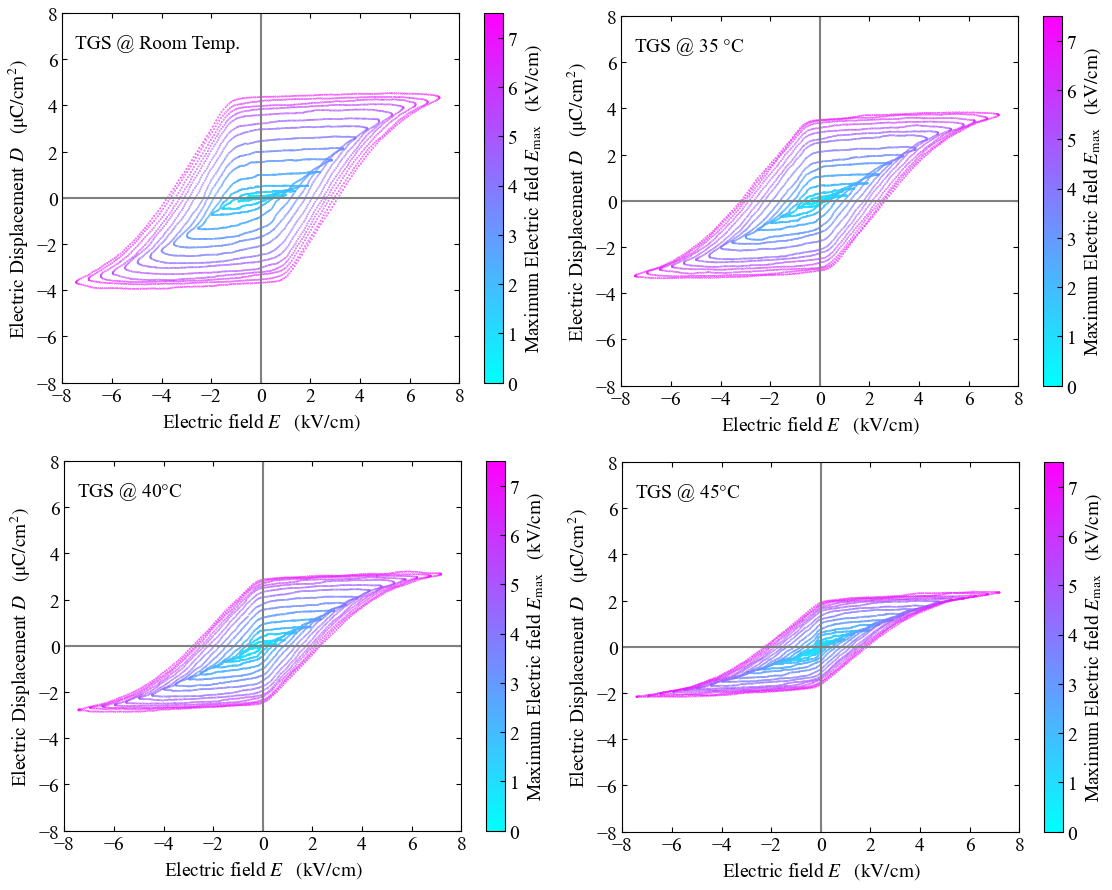
\includegraphics[width=\columnwidth]{TGS_D-E_temp.png}
        \caption{\small{各温度において、試料にかける最大電場を変えたときのヒステリシスループ。
        横軸が試料にかかっている電場\(E\), 縦軸が試料の電束密度\(D\), 色がヒステリシスループの最大電場を表している。}}
        \label{graph:TGS_D-E_Ec}
    \end{minipage}
    \hfill
    \begin{minipage}{0.4\columnwidth}
        \centering
        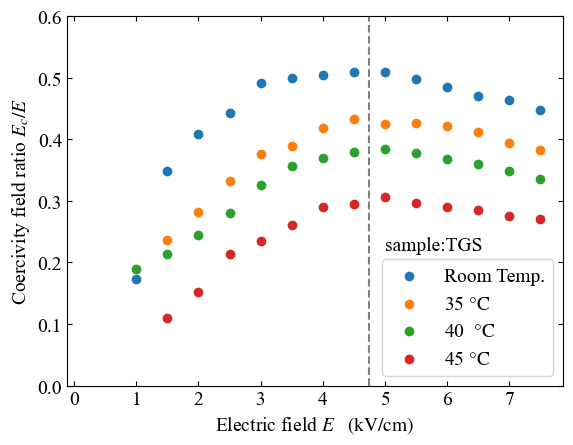
\includegraphics[width=\columnwidth]{TGS_Ec-E.png}
        \caption{\small{試料の電束密度が0となる電場の強さ(保持電場)\(E_c\)の温度特性。
        横軸をヒステリシスループの電場の最大値\(E\), 縦軸を\(E/E_c\)としている。}}
        \label{graph:TGS_Ec-E}
    \end{minipage}
\end{figure}

\begin{figure}[H]
    \begin{minipage}[t]{0.48\columnwidth}
        \centering
        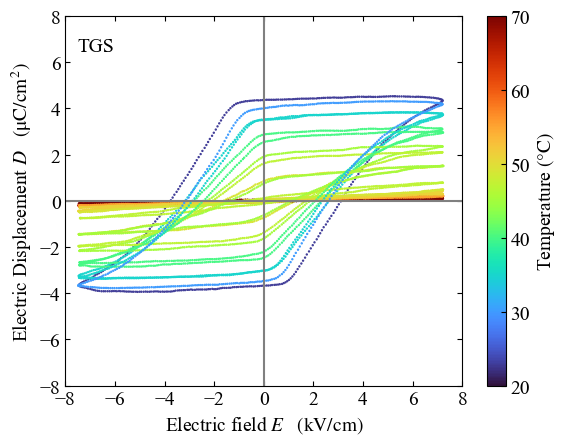
\includegraphics[width=\columnwidth]{TGS_D-E.png}
        \caption{\small{試料に書ける最大電場を 7.5 kV/cm としながら温度を変えたときのヒステリシスループの様子。
        色が温度を表している。
        50 \si{\degreeCelsius} 程度を境目にヒステリシスが潰れて直線状になっている。}}
        \label{graph:TGS_D-E_temp}
    \end{minipage}
    \hfill
    \begin{minipage}[t]{0.48\columnwidth}
        \centering
        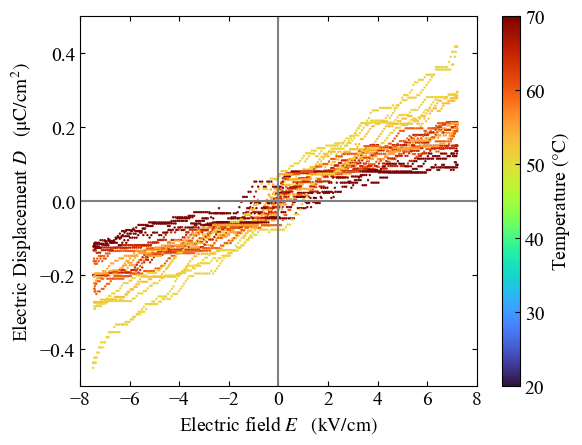
\includegraphics[width=\columnwidth]{TGS_D-E_para.png}
        \caption{\small{試料に書ける最大電場を 7.5 kV/cm としながら温度を変え、直線状になる温度領域でのヒステリシスループの様子。}}
        \label{graph:TGS_D-E_temp_para}
    \end{minipage}
\end{figure}

最大電場が 7.5 kV/cm 程度の入力電場のもとで温度を変えていったときのヒステリシスループの様子は図\ref{graph:TGS_D-E_temp}のようになった。
温度が上がると、ヒステリシスループがつぶれていき、
50 \si{\degreeCelsius} を境目にヒステリシスループがつぶれて直線状になっている。
これは電場をかけずとも分極が残る強誘電相から、入力電場に応じて分極が生じる常誘電相への相転移が生じている。
直線状になっている部分を拡大して表示したのが図\ref{graph:TGS_D-E_temp_para}である。
おおよそ直線状になっているなっているものの、がたつきが見られる。
移動平均を取る前のデータを確認するとこれはオシロスコープのレンジ設定が悪く、分解能が足りていないのが原因である。

\section{Discussion (TGS)}
\subsection{ランダウ理論}
ランダウ理論は系の自由エネルギーを系の対称性を顧慮しつつ相転移の様子を表す秩序変数を用いて表すことで、
自由エネルギー最小の原理と関数の形から相転移を記述するものである。
例えば反転対称のある系強磁性・常磁性相転移であれば秩序変数は磁化\(M\)で反転対称性より自由エネルギーは\(M^2\)の冪で書けることから
\begin{align}
    F = F_0 + a(T)M^2 + \frac{b(T)}{2}M^4 \cdots
\end{align}
のように書くことができる。ただし、自由エネルギーが最小になるという条件から最高次の係数は\(b(T)>0\)でなければならない。

TGS の結晶の空間群は\(P2_1\)であり、b 軸に関して自発磁化を持つ。
強誘電・常誘電相転移では結晶のひずみも関わ和ってくることが知られているのでこのひずみをヴォイトの表記を使って\(u_i,\,(1\leq i \leq6)\)と書くことにする。
秩序変数は分極\(p\)とひずみ\(u\)であり、自由エネルギーは
\begin{align}
    F
    &= F_0 + \frac{\alpha}{2}p_2^2 + \frac{\beta'}{4}p_2^4+\frac{1}{2\chi_1}p_1^2+\frac{1}{2\chi_3}p_3^2 + w \notag\\
    &+(Q_{21}u_1+Q_{22}u_2+Q_{23}u_3 + Q_{25}u_5)p_2^2 \notag\\
    &+(Q_{64}u_4+Q_{66}u_6)p_1 p_2 +(Q_{44}u_4+Q_{46}u_6)p_3 p_2+\cdots
\end{align}
と書ける\cite{ishibashi}。
第1行目の第3, 4 項はa軸とc軸の分極による項(\(\chi\)は電気感受率)
第2, 3行はひずみと分極の結合項である。
\(w\)は弾性エネルギーでありその中身は単斜晶であることを考慮して
\begin{align}
    w
    &= \frac{c_{11}}{2}u_1^2 + \frac{c_{22}}{2}u_2^2 + \frac{c_{33}}{2}u_3^2 + \frac{c_{44}}{2}u_4^2 + \frac{c_{55}}{2}u_5^2 + \frac{c_{66}}{2}u_6^2 \notag\\
    &\quad + c_{13}u_1u_3 + c_{12}u_1u_2 + c_{23}u_2u_3 +c_{15}u_1u_5 +c_{25}u_2u_5 +c_{35}u_3u_5 +c_{46}u_4u_6
\end{align}
となる。
これから平衡条件\(\partial F/ \partial u_i = 0\)を使うと\(u_1,\,u_2,\,u_3,\,u_5 \propto p_2^2\)がわかり、
さらに\(\partial F/ \partial p_1, \partial F/ \partial p_3 = 0\)を使うと\(u_4,\,u_6,\,p_1,\,p_3 = 0\)がわかる。
なので\(\beta'\)を取り直すことで
\begin{align}
    F = F_0 + \frac{\alpha}{2}p_2^2 + \frac{\beta}{4}p_2^4
\end{align}
というように自由エネルギーを取り直すことができる。

\(\partial F/ \partial p_2 = 0\)の平衡条件を考えると
\begin{align}
    \beta p_2 \qty(p_2^2+\frac{\alpha}{\beta})=0
\end{align}
となる。\(\beta > 0\)より\(\alpha<0\)であれば\(p_2\)は有限の値を持つことがわかる。
その有限の値\(p_2^2 = -\alpha/\beta\)をもとの自由エネルギーの式に入れると
\begin{equation}
    F' = F_0 -\frac{\alpha^2}{4\beta}
\end{equation}
より\(p_2=0\)のときの自由エネルギーの値より小さくなることがわかる。
自由エネルギー最小の原理と合わせると\(p_2\)が有限の値を持つときにはこの値が実現されることが言える。
つまり\(\alpha<0\)では結晶が b 軸方向に自発分極を持ち、\(\alpha>0\)では自発分極を持たないことを表している。
これより結晶の対称性だけで TGS が b 軸に自発分極を持つことが示せた。

簡単のため\(\beta\)は一定の値であるとして、\(\alpha\)のみが温度の依存性を持つとする。
強誘電相から常誘電相へ変化する温度であるキュリー温度を\(T_c\)としたとき、\(\alpha\)の符号が\(T_c\)で変わるような最も単純な関数形は
\(\alpha = a(T-T_c)\)である。そうすると自発分極の温度依存性が
\begin{align}
    p_2(T) = \pm a(T-T_c)^{1/2}
\end{align}
であると分かる。
この振る舞いは今回の測定結果(図\ref{graph:TGS_Ps-T})と合致している。
系の対称性からここまで説明できるのは興味深い結果である。

\subsection{保持電場\(E_c\)の温度特性}
試料の温度を変えたときのヒステリシスループの\(D=0\)との交点を調べることで保持電場\(E_c\)の温度依存性を読み取ることができる。
それをプロットすると図\ref{graph:TGS_Ec-T_temp}のようになった。昇温過程と降温過程で振る舞いが違うのがわかる。
冷却過程での温度計の示す値の様子を述べると、数値は単調に減少せずに時々上昇するような振る舞いが見られた。
ゆっくり冷却をしていった場合は試料全体の温度は均一で、試料から熱が逃げていくので温度計の示す値は単調に減少していく。
一方、冷却が速く試料中央と表面で温度差があるとき、表面付近にある温度計は試料の内部からの熱の流入と外部への熱の流出との両方の影響を受けるため、
温度計の示す値は上下する。
つまり冷却時のデータは試料自身の温度と温度計の温度のずれが大きくなっているためあまり信用できないというのがわかる。

なので昇温過程過程のデータのみを考察で考える。
図\ref{graph:TGS_Ec-T_temp}の強誘電相でのカーブを\(E_c\propto(T_c-T)^a\)でフィッティングすると、\(T_c =\) 51.7\si{\degreeCelsius},
\(a =\) 0.36 になった。
\begin{figure}[H]
    \begin{minipage}[t]{0.48\columnwidth}
        \centering
        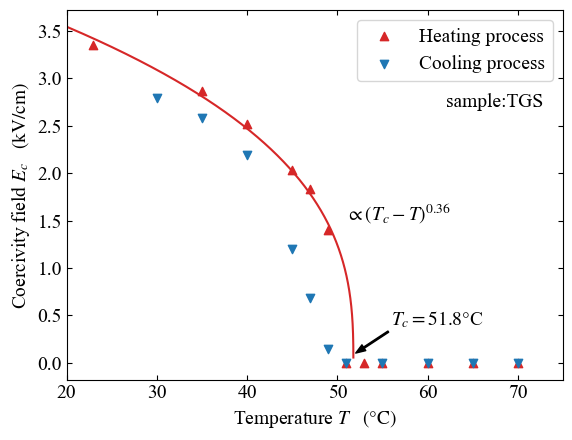
\includegraphics[width=\columnwidth]{TGS_Ec-T.png}
        \caption{\small{保持電場\(E_c\)の温度依存性。
        昇温過程と降温過程でふるまいが違うのは測定に失敗したのが原因。}}
        \label{graph:TGS_Ec-T_temp}
    \end{minipage}
    \hfill
    \begin{minipage}[t]{0.48\columnwidth}
        \centering
        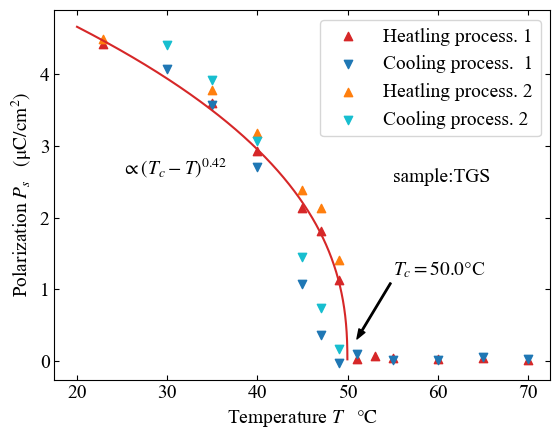
\includegraphics[width=\columnwidth]{TGS_Ps-T.png}
        \caption{\small{自発\(P_s\)の温度依存性。
        ヒステリシスループから求める方法が2つあり(考察)それぞれの方法を1, 2 としている。}}
        \label{graph:TGS_Ps-T}
    \end{minipage}
\end{figure}

この結果をランダウ理論と比較する。
この系において、外場\(E\)があるときの自由エネルギーは
\begin{align}
    F = F_0 + \frac{\alpha}{2} p_2^2 + \frac{\beta}{4} p_2^4 -p_2E
\end{align}
となる。平衡条件\(\partial F/\partial p_2 = 0\)より
\begin{align}
    \alpha p_2 + \beta p_2^3 - E = 0
\end{align}
保持電場\(E_c\)は\(dp/dE\)が発散するような\(E\)のことである。
この式を\(E\)で微分することによりこのときの分極\(p_c\)が得られる。
\begin{align}
    &(\alpha+3\beta p^2)\dv{p}{E} = 1 \\
    &\quad \rightarrow p_c^2 = \frac{-\alpha}{3\beta}
\end{align}
よって保持電場\(E_c\)は
\begin{align}
    E_c = \alpha p_c + \beta p_c^3 = \pm\sqrt{\frac{-4\alpha^3}{27\beta}} \propto (T_c-T)^{3/2}
\end{align}
となる。

指数が完全に違うことから、保持電場を考える際には結晶の対称性以外の要素を取り入れなければならないことがわかる。
そうしたときに考えられる要因としては試料の結晶性が悪く、不純物や欠陥を考慮しなければならないという点である。
これにより分域の動き方が制限されるといったものであるが、
これはバルクハウゼン効果としてヒステリシスループがわずかにがたつくといった要素として合わられると考えられるためここでは考えにくい。

ほかの要素として考えられるのは分域同士の双極子双極子相互作用によって分域の反転が生じにくくなるという機構が考えられる。
% TODO: たしか分域構造とトポロジカル物性ってなんか関係あったよね。
% TGS の b軸方向の自発分極ってことは低次元系とみなせるかもしれないしそういう話がありそう。
分域内部の単位胞内での電子の偏りによる双極子モーメントは a軸c軸平面内の隣接する単位胞にある電子との重なり積分により生じているが、
分域構造のスケールでは量子力学的効果が失われ古典的な双極子双極子相互作用が支配的になる。
なので外部電場を加えようとも分域同士の双極子相互作用によって反強誘電性的な構造の保護が生じるため、
\(E_c\)の臨界指数がランダウ理論の予言よりも小さくなると考えられる。

ここの\(E_c\)付近では分域構造が反強誘電性のように見えるという視点は興味深いものである。
Ferro 的な試料であっても適切な履歴のもと\(E_c\)に相当する外場を加えるとこの近傍では antiFerro 的な振る舞いを見せることとなる。
このように考えると antiFerro 的な状況でしか見つからないとされた現象が Ferro 的な物質でも引き起こすことができるため、
探索できる物質が増えるのではないかと考えられる。

\subsection{自発分極\(P_s\)の求め方1}
強誘電体であることを特徴づける自発分極\(P_s\)をヒステリシスループから求めることを考える。
電束密度\(D\)と電場\(E\), 分極\(P\)の間の関係は
\begin{align}
    D = \varepsilon_0 E + P
\end{align}
である。これより\(E=0\)における電束密度の値が自発分極となる。
しかし実際には分域構造のため、\(E=0\)出の電束密度\(D\)の値は自発分極\(P_s\)をそのまま表してはいない。
そのため、工夫をする必要がある。

その方法の1つが\(E\)が十分大きいときから\(E\)が減少していく過程の部分を線形近似し、その直線の外挿によって求める方法である。
\(E\)が十分大きいときには分域構造はなく、自発分極はすべて同じ向きを向いていると考えられるので、
電束密度\(D\)と電場\(E\), 分極\(P\)の間の関係式のうち\(P\)は一定となり、直線となる。
なのでこの領域を線形近似すると、直線の傾きが誘電率、切片が自発分極となる。
この方法を使って自発分極\(P_s\)を求めたのが図\ref{graph:TGS_Ps-T}の1と付いているデータである。

この方法は最も素直な自発分極の導出の仕方であるが、測定データが多く、Excel で解析をするとなるとあまりにも煩雑で
なおかつ線形近似を取る範囲の基準が不明瞭であることから自動化することも難しく、データ処理をする観点からはあまり良いものではないと考えられる。

\subsection{ヒステリシスロス\(\Delta\)の温度特性とこれを利用した自発分極\(Ps\)の求め方}
ヒステリシスループの面積\(\Delta\)はこのヒステリシスループを一周するのに必要なエネルギーである。
これを求めるのに閉曲線を構成する座標\((x_n,\,y_n)\)が与えられたときにその閉曲線の内側の面積を求める公式
\begin{align}
    S = \frac{1}{2}\abs{\sum_n \qty(x_n y_{n+1} - x_{n+1}y_n)}
\end{align}
を利用して求めた。この公式はグリーンの公式を離散化したものに相当する。
これをプロットすると図\ref{graph:TGS_Delta-T}のようになった。

ここでヒステリシスループの形状に注目するとおおよそ平行四辺形となっていることから
\begin{align}
    \Delta = 4 E_c P_s
\end{align}
になることが期待され、実際に強誘電相で最大電場を変えたときのこの比率をプロットすると図\ref{graph:TGS_Delta-E}のようになる。
確かに比率はほとんど 1 になっていてこの式が使えることがわかる。

つまり逆にいうとヒステリシスループの面積\(\Delta\)と保持電場\(E_c\)を求めさえすれば自発分極\(P_s\)の値が出ることになる。
この方法で求めたのが図\ref{graph:TGS_Ps-T}の2と付いているデータである。
別の方法で求めたのにも関わらず同じ振る舞いをしているのがわかる。

ヒステリシスループの面積\(\Delta\)はその試料全ての自発分極を反転させるのに必要なエネルギーのことであるので試料特有の量であり、
\(E_c\)もその試料特有の分域構造を反映した温度特性を示す。
なのでこれはヒステリシスループの形状が平行四辺形からずれたときにも使えることが予想される。
これは後ほどBTOの結果についてでも言及する。

\begin{figure}[H]
    \begin{minipage}[t]{0.48\columnwidth}
        \centering
        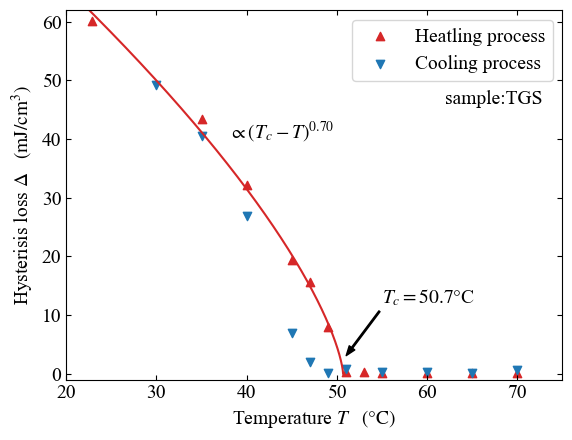
\includegraphics[width=\columnwidth]{TGS_Delta-T.png}
        \caption{\small{ヒステリシスループの面積(ヒステリシスループを一周するのに必要なエネルギー)の温度特性}}
        \label{graph:TGS_Delta-T}
    \end{minipage}
    \hfill
    \begin{minipage}[t]{0.48\columnwidth}
        \centering
        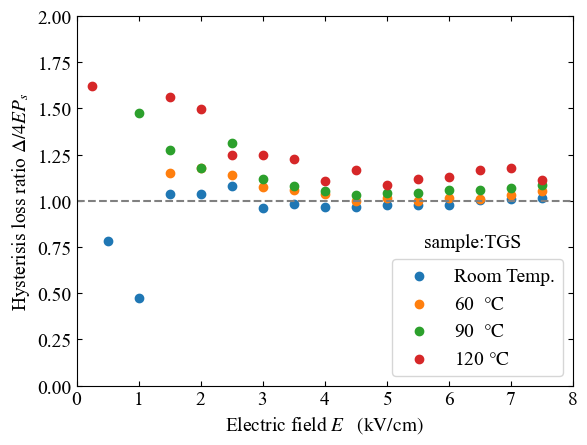
\includegraphics[width=\columnwidth]{TGS_Delta-E.png}
        \caption{\small{ヒステリシスループの面積\(\Delta\)と保持電場\(E_c\), 自発分極\(P_s\)の間の関係。
        \(\Delta=4E_cP_s\)が成り立っているのがわかる。}}
        \label{graph:TGS_Delta-E}
    \end{minipage}
\end{figure}

% \subsection{比誘電率}
% 実験的には誘電率は
% \begin{align}
%     \varepsilon = \pdv{D}{E}
% \end{align}
% で求められる量である。
% 常誘電相であれば自発分極はないので得られた\(D-E\)応答の傾きをそのまま求めればよい。
% 一方強誘電相のとき、ヒステリシスループの傾きは一定ではなく、どの傾きを取ればよいかはわからない。
% ひとまず、\(E=0\)のときの傾きを取ることにしてプロットしたのが図\ref{graph:TGS_epsilon-T}である。
% \begin{figure}[H]
%     \begin{minipage}[t]{0.48\columnwidth}
%         \centering
%         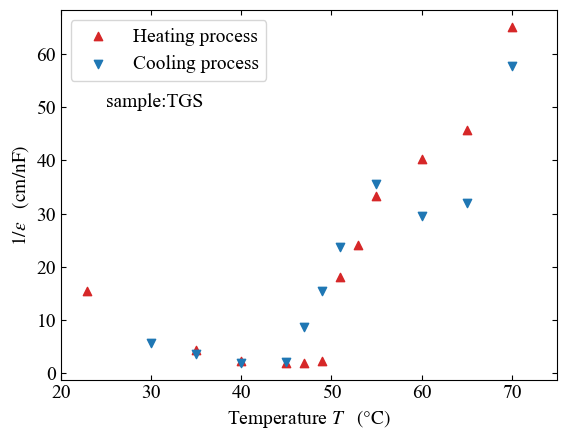
\includegraphics[width=\columnwidth]{TGS_epsilon-T.png}
%     \end{minipage}
%     \hfill
%     \begin{minipage}[t]{0.48\columnwidth}
%         \centering
%         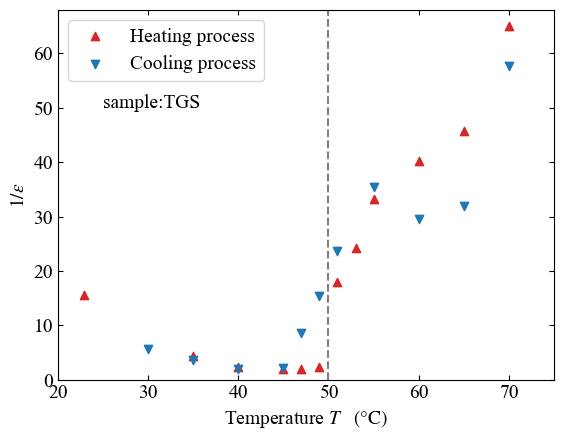
\includegraphics[width=\columnwidth]{TGS_epsilon1-T.png}
%     \end{minipage}
%     \caption{\small{誘電率の温度特性。破線が強誘電相と常誘電相の境目で各相によって求め方が異なっている。}}
%     \label{graph:TGS_epsilon-T}
% \end{figure}


\section{Results (BTO)}

\section{Discussion (BTO)}
% \subsection{強誘電・常誘電相転移の機構}
% BTOでの相転移はペロブスカイトの構造による格子振動とクーロン相互作用の結合による構造の不安定化によるものである。
% %仮置き
% 格子振動は電荷の偏りを生じる光学モードと偏りを生じない音響モードの2つがある。
% 光学モードにおける電荷の偏りはつまり分極と解釈できる。
% 分極は外部電場と結びつくため云々。

\section{Conclusion}


\bibliographystyle{junsrt}
\bibliography{reference}
\nocite{*}

% \appendix
% \section{点群・空間群}
% 結晶に対称性があるといったとき、
% それは結晶を回転させたり、鏡映しにしたりしてもその格子点の配置が変わらないということによって特徴づけできる。
% つまりある操作が与えられたときにその結晶の格子点の配置が変わるか変わらないかで結晶を分類することができる。

% 結晶全体を平行移動させる並進操作によって

% % 結晶を対称性によって分類し、その性質を見ていくのに数学における群論という代数が適している。
% % 集合\(G\)とその上の二項演算\(\cdot\)の組が群であるとは次の3つの条件を満たすことをいう。
% % \begin{itemize}
% %     \item 任意の\(G\)の元 \(g,\,h,\,k\)に対して\(g\cdot(h\cdotk) = (g\cdot h) \cdot k\)
% %     \item 任意の\(G\)の元 \(g\) であっても \(e\cdot g = g\cdot e = g\)を満たすような\(G\)の元\(e\)が存在する。
% %     \item 任意の\(G\)の元 \(g\) に対して \(g \cdot g^{-1} = g^{-1}\cdot g = e\)となるような\(G\)の元\(g^{-1}\)が存在する。
% % \end{itemize}
% % 群の例として、整数\(\mathbb{Z}\)は加法に関して群であり、
% % 逆行列が非負の\(n\times n\)行列全体\(GL(n,\mathbb{R})\)は行列の積に関して群である。
% これを


% \section{結晶の対称性と Ginzburg-Landau 理論}

\end{document}